\chapter{Methodology}
	\section{Agile Method as Software Development Model}
	Building overall project in python and implementing in android smartphone was a big challenge which can be made easy by building project with a small section and developing it to a fully functioned project. Implementing the whole project inside android app was a challenging part as the processing power and efficiency of mobile device could be compromised. Therefore Agile model was used as Software Development model as it facilitied us to start our project from a small section and launch it as beta version which helped us to visualize where the project was going and which part it had defect.\\
	\begin{figure}[h]
		\centering
			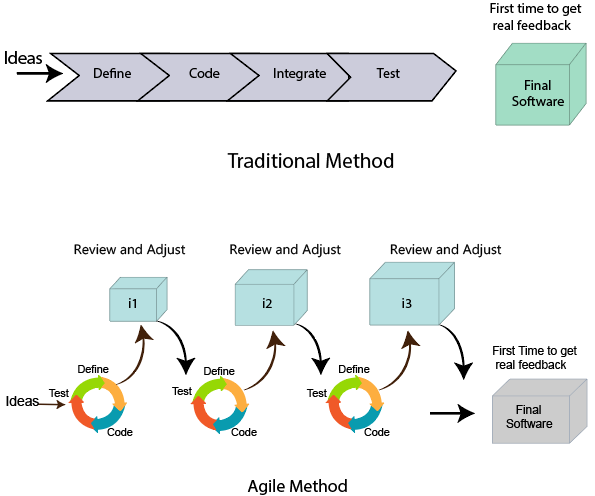
\includegraphics[width=0.8\textwidth]{img/agilem.png}
			\caption{Agile Model as Software Development Model}    
		\end{figure}
	\break
	\section{Asana as Kanban Board}
	Asana was used as Kanban Board to organize, distribute, manage and track all the works and tasks assigned to each members of our team. All the works done in base level as well as the meeting minutes were recorded in Asana.\\
	\begin{figure}[h]
		\centering
			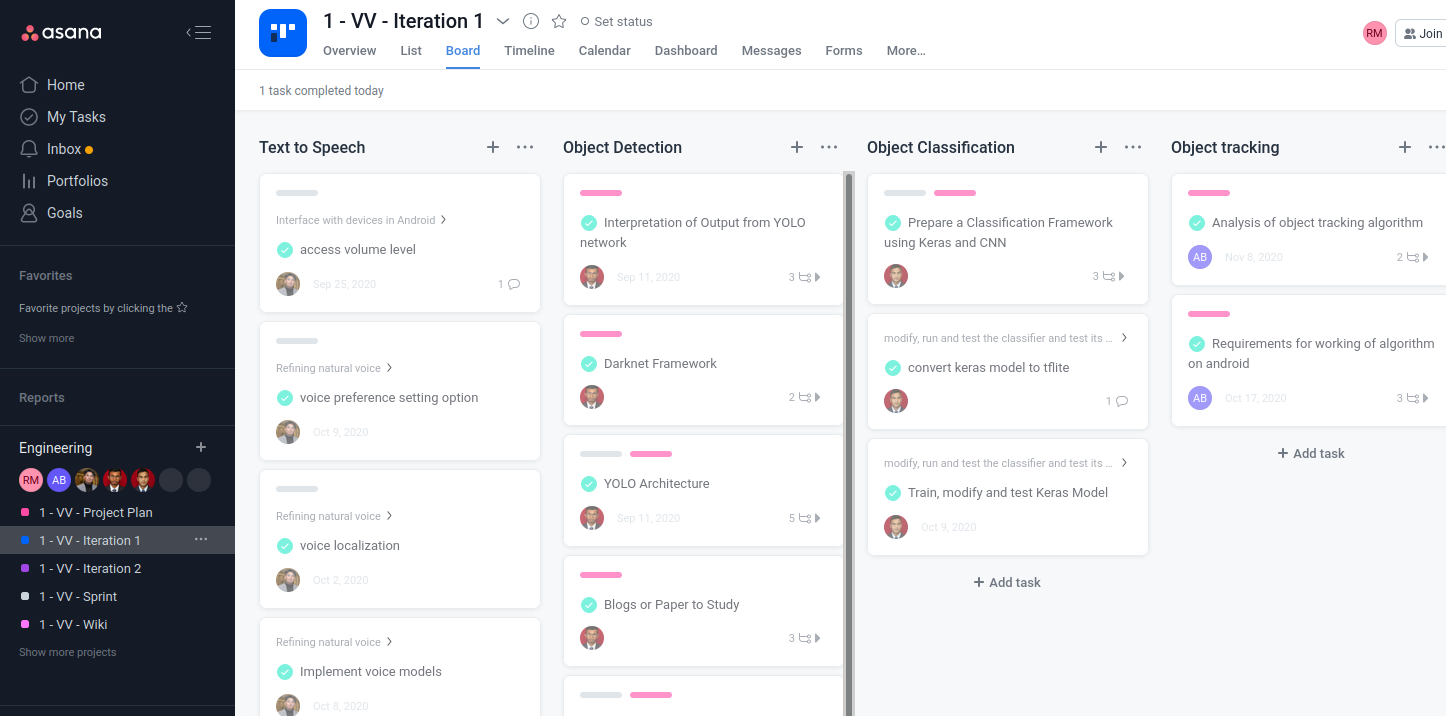
\includegraphics[width=1\textwidth]{img/asana.png}
			\caption{Asana}    
	\end{figure}
	The Project was managed in asana in five sessions:
		\subsection{Project Plan}
			Planning for further steps were done in detail in this session. All the tasks to be done, their sub tasks, deadline of the tasks and subtasks were recorded here. Then the task was linked to respective iteration session by the assigned member before doing the task.
		\subsection{Sprint}
			The works decided to be done, being done and the one that were done recently were recorded here.
		\subsection{WIKKI}
			Utility tasks that are useful and informative but unrelated to the actual project were listed here. Forexample: tutorials and guidelines to use gitlab, asana, etc were listed here.
		\subsection{Iteration1}
			Everything related to the first iteration of our project were recorded here including meeting minutes and reports.
		\subsection{Iteration2}
			Everything related to the second iteration of our project were recorded here including meeting minutes and reports.
	\section{Overall Phase Followed}
	The overall project has been completed in three main phase which are:
	\begin{enumerate}
		\item Planning Phase
		\item Development Phase
		\item Integration
	\end{enumerate}
	\subsection{Planning Phase}
	In planning phase, necessary works to be done and planning of overall project were discussed and the decision were documented for further procedures.\\
	First the project was divided into four parts:
	\begin{enumerate}
		\item Image detection
		\item Image classification
		\item Imge Tracking
		\item Text to Speech
	\end{enumerate}
	These parts were then assigned to each project members who then studied about the respective parts in detail.
	\subsection{Development Phase}
	In this phase, the divided parts were well studied and developed. Then each of those developed parts were tested separately.
	\subsection{Integration}
	In this phase, the separately developed parts were integrated to form a system and integration testing was done.\pagebreak
	\section{Task Workflow}
	Each tasks of every session were done and recorded in a procedural manner and the programmes were recorded and stored in gitlab.\\
	The workflow of the tasks follow following steps:
	\begin{enumerate}
		\item Get task assigned in Asana
		\begin{figure}[h]
			\begin{center}
				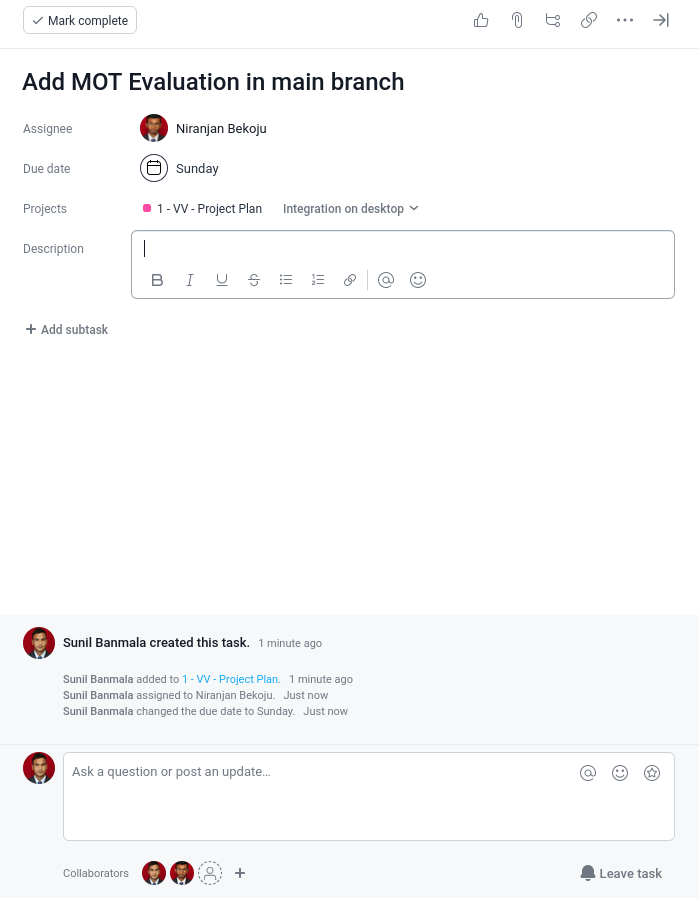
\includegraphics[width=0.5\textwidth]{img/asana_create_task.png}
			\end{center}
			\caption{Create task in asana}    
		\end{figure}
		\item Create issue in gitlab for each tasks assigned to self
		\begin{figure}[h]
			\begin{center}
				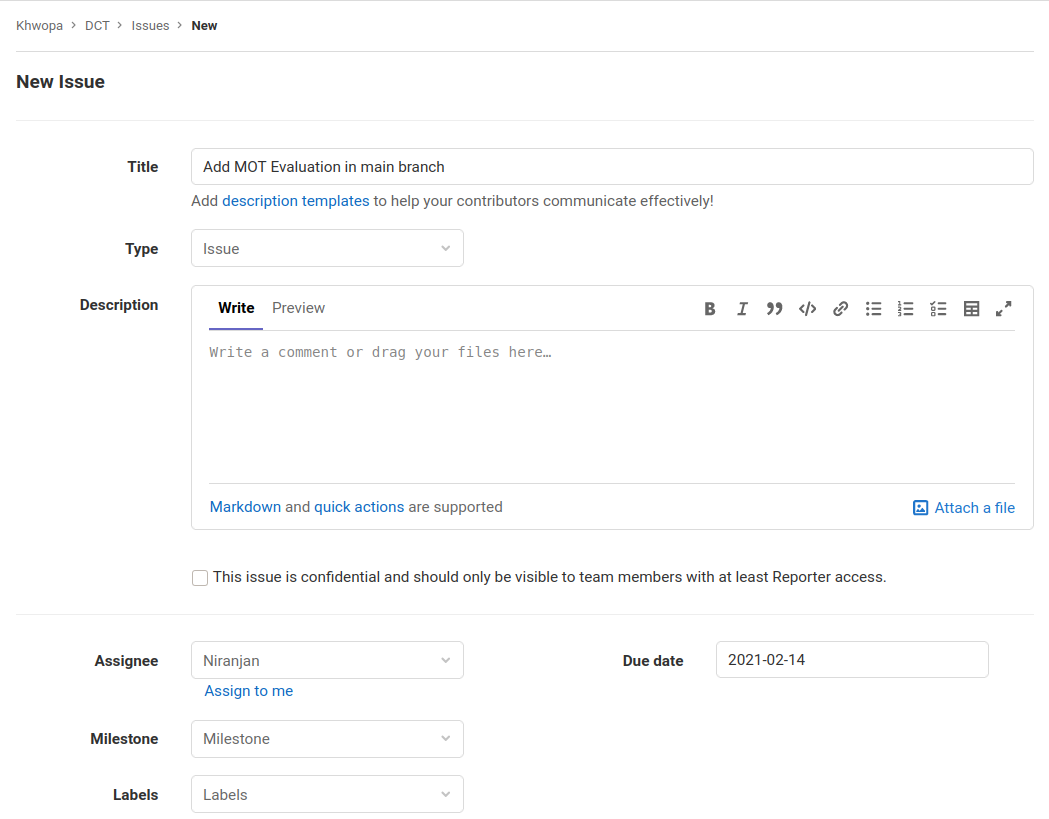
\includegraphics[width=0.5\textwidth]{img/gitlab_create_issue.png}
			\end{center}
			\caption{Create issue in gitlab}    
		\end{figure}\\
		\item Create corresponding branch in gitlab and fetch the branch in local
		\item Checkout to the branch and do assigned tasks there
		\item Then push the task done, to the gitlab
		\item Mark the task assigned in Asana to: Done
	\end{enumerate}